\subsection{Diskretisering av skip}
Nå ser vi på diskretisering av den våte delen av en rektangulær geometri. Dypgangen $D$ velges som enhetslengde i problemet, og $L$ er lengden. Vi har fire geometrier. $L/D = 10, 2,1, \text{0,1}$

\noindent
\begin{minipage}[t]{0.45\linewidth}
    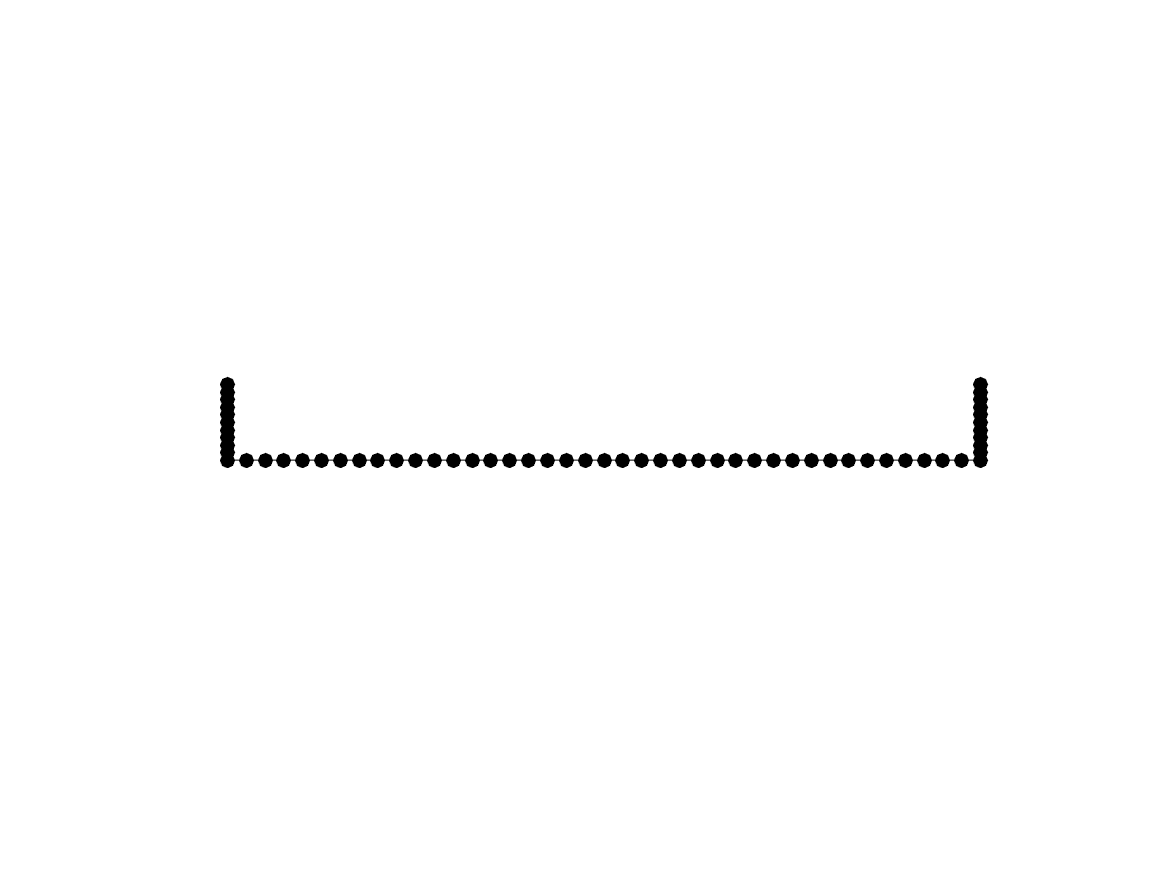
\includegraphics[width=\linewidth]{/Users/ole/Tex/MEK4420/oblig2images/boxes_1.png}
    \captionof{figure}{L/D = 10}
\end{minipage}
\hspace{0.05\linewidth}
\begin{minipage}[t]{0.45\linewidth}
    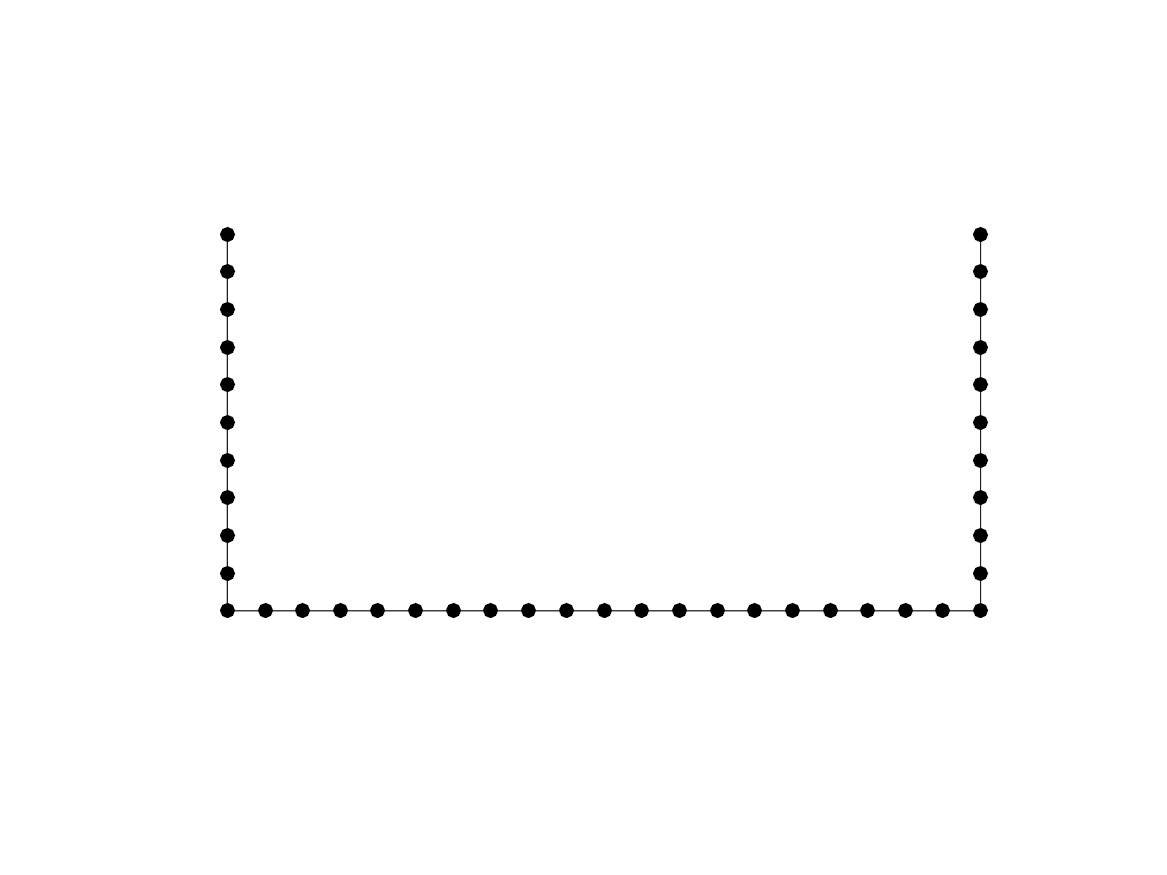
\includegraphics[width=\linewidth]{/Users/ole/Tex/MEK4420/oblig2images/boxes_2.png}
    \captionof{figure}{L/D = 2}
\end{minipage}

\vspace{0.5cm} % Adds vertical space between rows

\noindent
\begin{minipage}[t]{0.45\linewidth}
    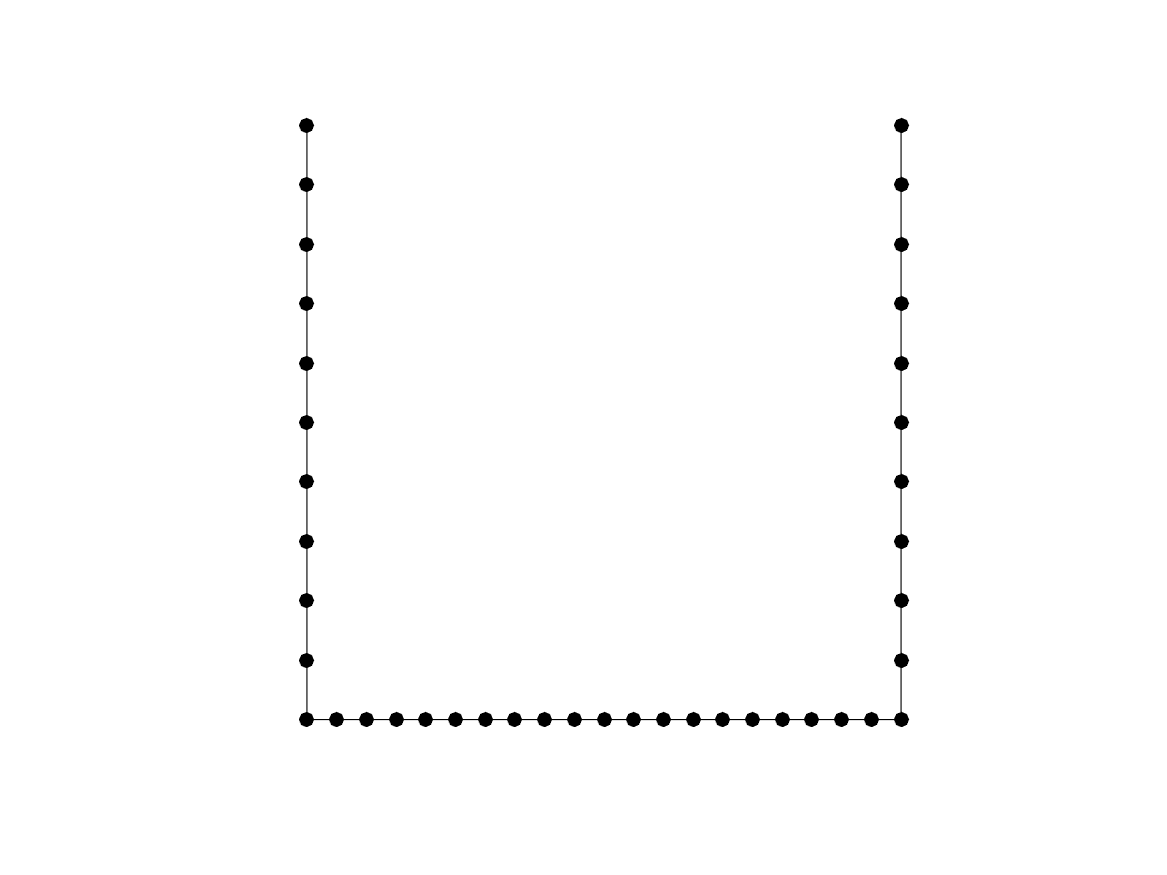
\includegraphics[width=\linewidth]{/Users/ole/Tex/MEK4420/oblig2images/boxes_3.png}
    \captionof{figure}{L/D = 1}
\end{minipage}
\hspace{0.05\linewidth}
\begin{minipage}[t]{0.45\linewidth}
    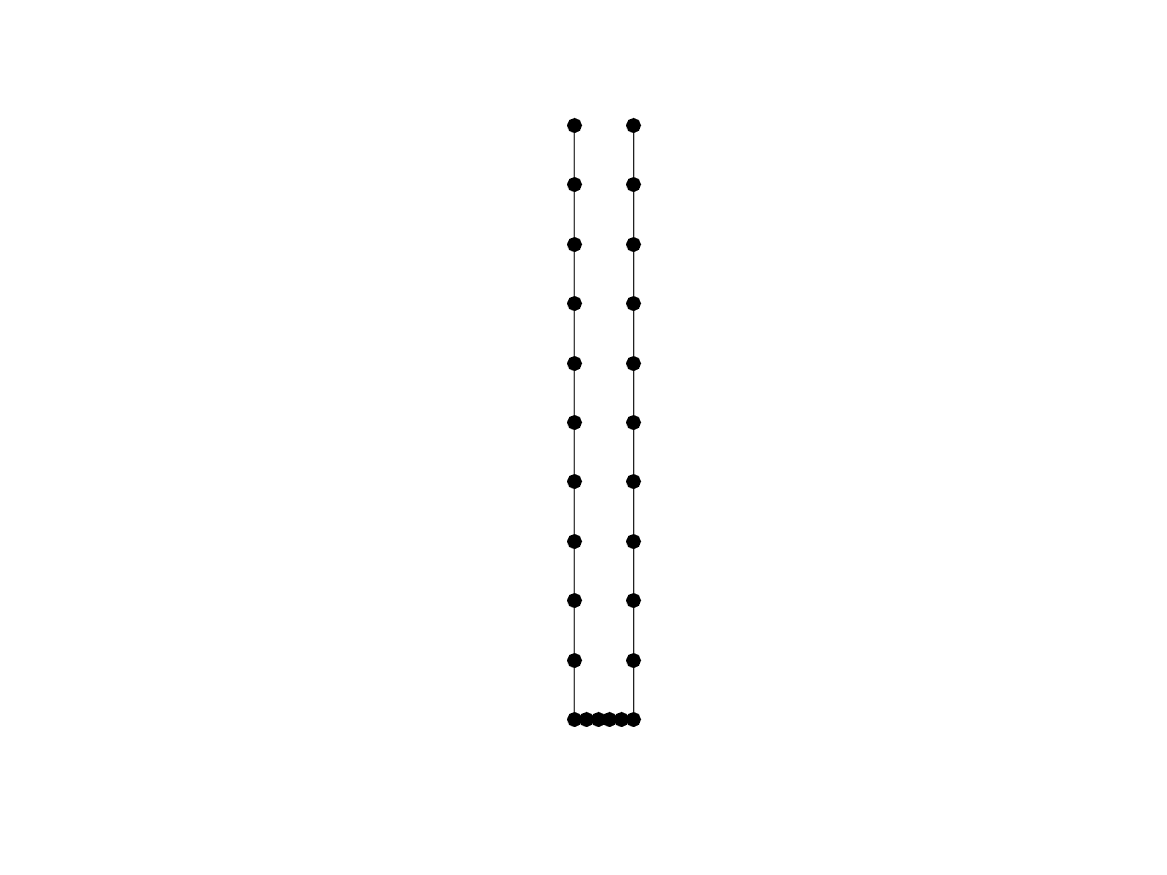
\includegraphics[width=\linewidth]{/Users/ole/Tex/MEK4420/oblig2images/boxes_4.png}
    \captionof{figure}{L/D = 0.1}
\end{minipage}



